\documentclass{article}
\usepackage[utf8]{inputenc}
\usepackage[english, swedish]{babel}

\usepackage{cite}
\usepackage{caption}
\usepackage{graphicx}
\usepackage{float}
\usepackage{textcomp}
\usepackage[yyyymmdd]{datetime}
\renewcommand{\dateseparator}{-}

\usepackage{graphicx}
\graphicspath{ {images/} }

%For headers & footers
\usepackage{fancyhdr}
\pagestyle{fancy}
\lhead{
\includegraphics[scale=0.2]{Logo}}
\chead{Kartrobot}
\rhead{\today}

\lfoot{Konstruktion med mikrodatorer}
\rfoot{Grupp 3}

\renewcommand{\headrulewidth}{0.4pt}
\renewcommand{\footrulewidth}{0.4pt}


\title{Designspecifikation för kartrobot}
\author{Patrik Sletmo}
\date{\today}

\selectlanguage{swedish}

\begin{document}

\thispagestyle{empty}

{
\sffamily
\centering
\large


{\huge 
Designspecifikation för kartrobot
}

{\large
Patrik Sletmo
}

{\large
Version 0.1
}

\vspace{3.5cm}

Status
\begin{center}
\begin{tabular}{ | c | c | c | } 
\hline
\end{tabular}
\end{center}
}
\clearpage

\vspace*{\fill}
{
\sffamily
\centering
\large


{\huge
Projektidentitet
}

{\large
Grupp 3, 16/HT, KarToffel \\ Linköpings tekniska högskola, institution
}

\vspace{0.5cm}

\begin{table}[H]
\centering
\begin{tabular}{ | c | c | c | c |}
\hline
Namn & Ansvar & Telefon & E-post \\
\hline
Patrik Sletmo & Projektledare & 070 783 57 61 & patsl736@student.liu.se \\
\hline
Rebecca Lindblom & Utvecklare & 073 436 40 79 & rebli156@student.liu.se \\
\hline
Matildha Sjöstedt & Utvecklare & 070 515 84 11 & matsj696@student.liu.se \\
\hline
Sebastian Callh & Utvecklare & 073 820 46 64 & sebca553@student.liu.se \\
\hline
Anton Dalgren & Utvecklare & 076 836 51 56 & antda685@student.liu.se \\
\hline
Matilda Dahlström & Utvecklare & 070 636 33 52 & matda715@student.liu.se \\
\hline
\end{tabular}
\end{table}
}

\begin{center}
\textbf{Hemsida}: https://github.com/SebastianCallh/kartoffel-tsea29
\end{center}

\begin{center}
\textbf{Kund}: Mattias Krysander, 013 - 28 2198 , matkr@isy.liu.se
\end{center}

\begin{center}
\textbf{Kursansvarig}: Tomas Svensson, 3B 528, +46 (0)13 28 1368, tomas.svensson@liu.se \\
\textbf{Handledare}: Anders Nilsson, 3B 512, +46 (0)13 28 2635, anders.p.nilsson@liu.se
\end{center}
\vspace*{\fill}
\clearpage

\renewcommand*\contentsname{Innehållsförteckning}
\tableofcontents
\clearpage


{
\sffamily
\centering
\large


{\huge 
Dokumenthistorik \\
}
\begin{center}
\begin{tabular}{ | c | c | c | c | c |} 
\hline
\textbf{Version} & \textbf{Datum} & \textbf{Utförda ändringar} & \textbf{Utförd av } & \textbf{Granskad} \\  
\hline
\end{tabular}
\end{center}
}

\clearpage


\section{Inledning}
% Kort beskrivning av hela dokumentet, skrivs förslagsvis sist

\clearpage

\section{Systembeskrivning}
% Beskrivning av systemets mest framträdande egenskaper
Systemet i sin helhet består av en fyrhjulig robot, vars uppdrag är att autonomt kartlägga ett rum. Roboten tar in data om omvärlden med hjälp av olika sensorer, bland annat IR- och lasersensorer. Denna data ger roboten underlag för att kartlägga rummet, samt ta beslut om framtida navigation.  

\subsection{Delsystem}
% Upplistning av delsystem, eventuellt någon kort kommentar om varje delsystem
Hela systemet är moduluppbyggt, och består av följande delsystem:
\begin{itemize}
\item Mjuvaruenhet
\item Huvudenhet
\item Sensorenhet
\item Styrenhet
\end{itemize}
Mjukvaruenheten är den enda enheten i systemet som inte är en fysisk del av själva roboten, utan uppträder i en bärbar dator. Dess uppgifter är att kommunicera med roboten via Bluetooth, till exempel för att möjliggöra manuell fjärrstyrning, samt att presentera befintlig kartdata i ett grafiskt gränssnitt till användaren.  
\newline\newline
Huvudenhetens uppgifter består dels av att sköta kommuntikationen, både i I2C-bussen till de två andra modulerna i roboten och via Bluetooth till mjukvaruenheten, samt att sköta all logik. Huvudenheten använder data från sensorerna för att kartlägga rummet samt för att ta beslut om hur den ska navigera till outforskade områden.
\newline\newline
Sensorenheten har som uppgift att sampla data from omvärlden med hjälp av dess sensorer, och tillhandahålla denna data när huvudenheten ber om dem.
Styrenhetens uppgift är att utifrån kommandon från huvudenheten föra roboten till vald position med hjälp av servon kopplade till robotens hjul. Styrenheten kontrollerar också det servo som lasersensorn är kopplad till, för att den ska kunna vridas och kunna mäta avstånd åt flera håll. 

\subsection{Övergripande konstruktion}
% Övergripande blockschema
\begin{figure}[H]
\centering
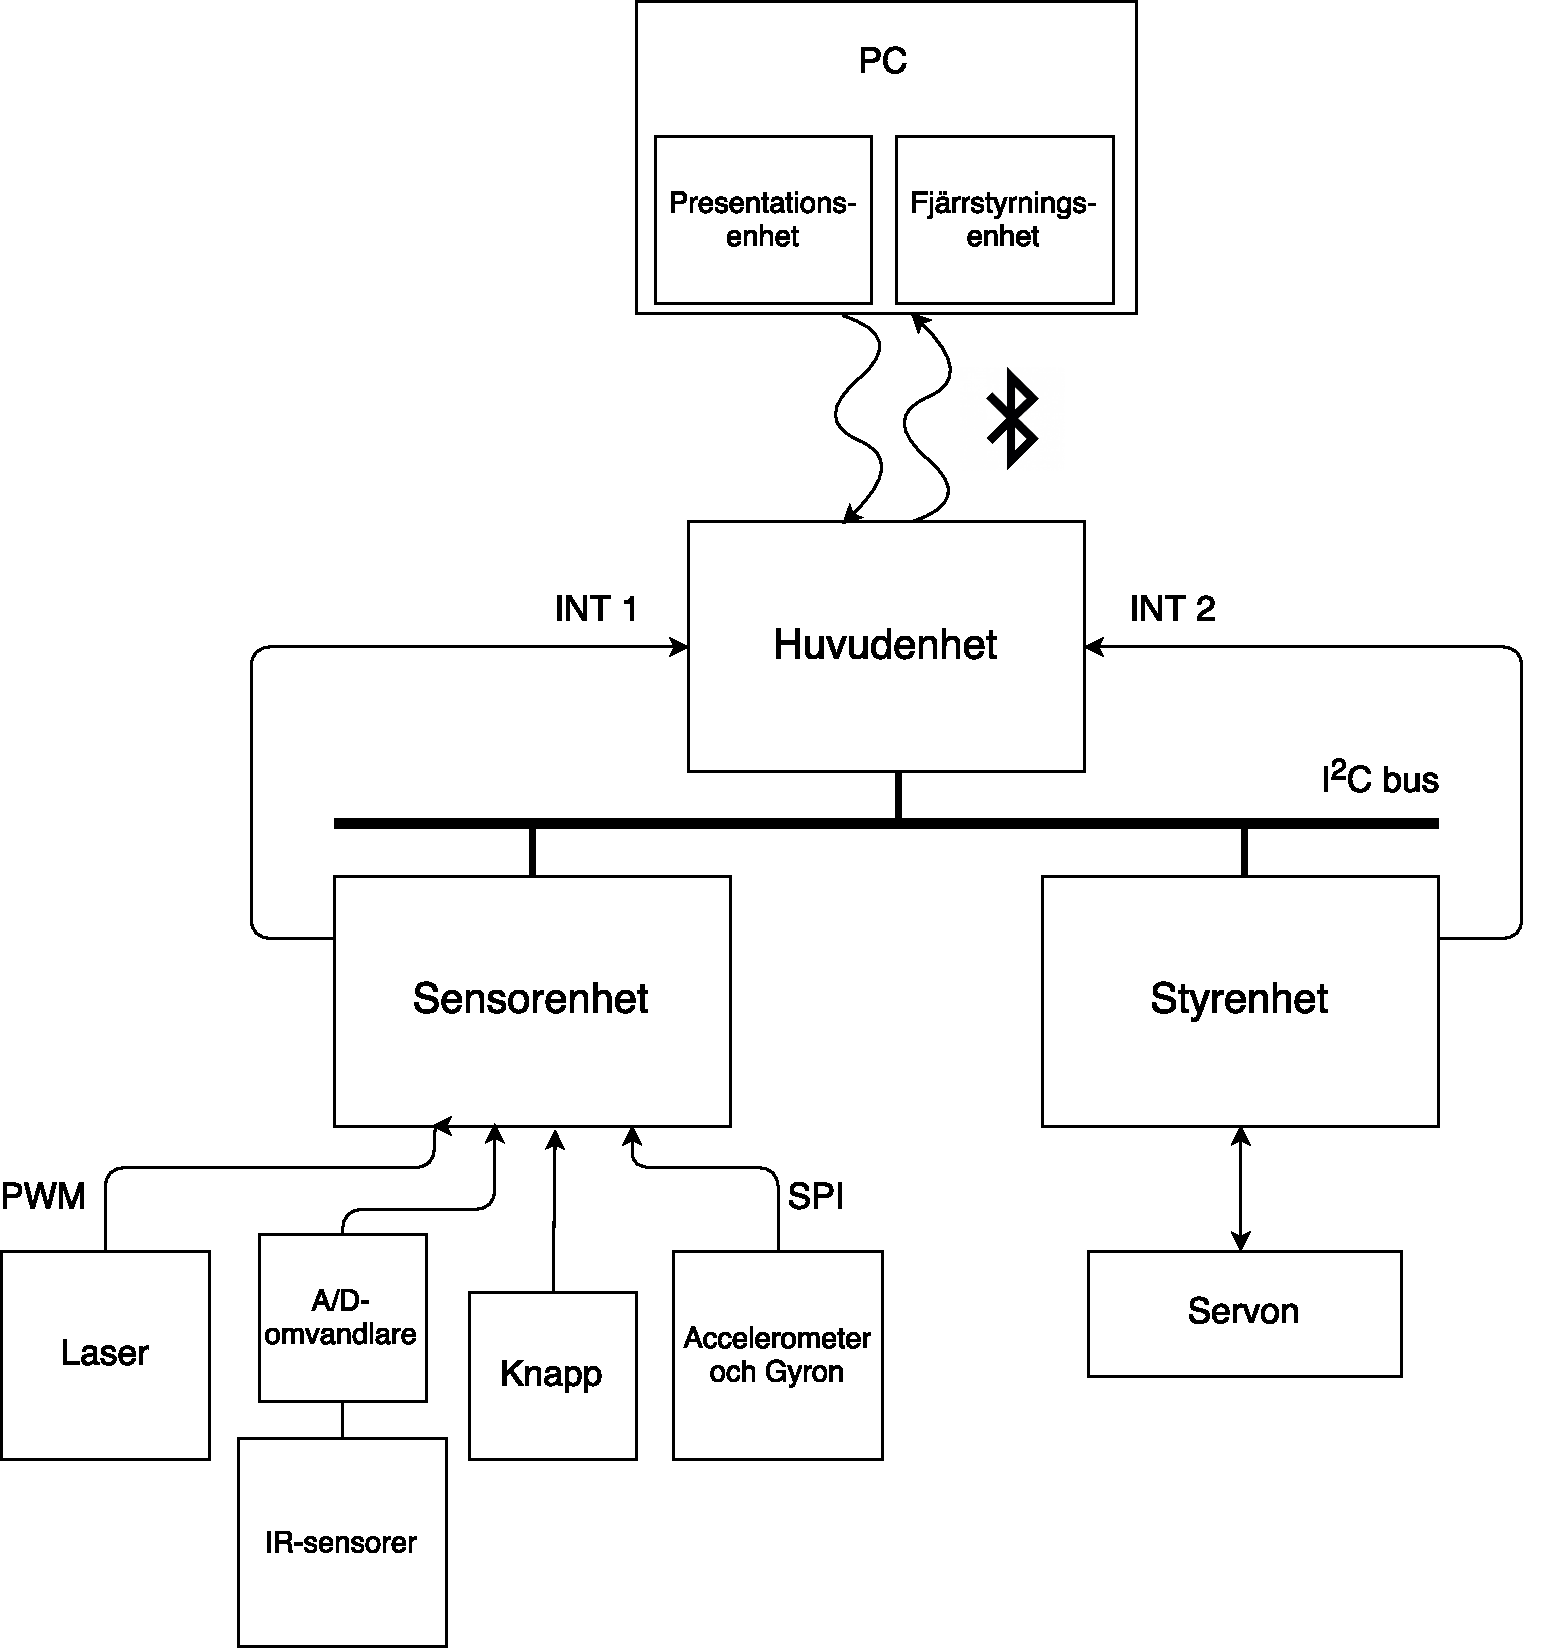
\includegraphics[scale=0.35]{oversikt_systemet2}
\caption{Översikt över systemet}
\label{fig:oversikt_systemet2}
\end{figure}

Ett övergripande blockschema av systemet visas i figur ~\ref{fig:oversikt_systemet2}.

\subsection{Komponenter}
% Väldigt kort beskrivning av delsektion
Här nedan listas alla komponenter som roboten kommer att vara del av roboten.

\subsubsection{Beräkningsenheter}
% Upplistning av processorer, SOC:s, etc
\begin{table}[H]
  \centering
  \begin{tabular}{ | c | c | c | c |}
    \hline
    \textbf{Enhet} & \textbf{Antal} \\
    \hline
    Raspberry Pi 3 & 1 \\
    \hline
    ATMega 1284 & 2 \\
    \hline
  \end{tabular}
  \caption{ Tabell över beräkningsenheter. }
\end{table}

\subsubsection{Sensorer}
% Upplistning av alla sensorer
\begin{table}[H]
  \centering
  \begin{tabular}{ | c | c | c | c |}
    \hline
    \textbf{Komponent} & \textbf{Antal} \\
    \hline
    LIDAR-Lite v2 & 1 \\
    \hline
    Knapp & 1 \\
    \hline
    GP2Y0A21 IR-Sensor & 2 \\
    \hline
    MLX90609 Gyro & 1 \\
    \hline
    MPU6050 Accelerometer + Gyro & 1 \\
    \hline
  \end{tabular}
  \caption{ Tabell över sensorer. }
\end{table}

\subsubsection{Ställdon}
% Servon, motorer, etc
\begin{table}[H]
  \centering
  \begin{tabular}{ | c | c | c | c |}
    \hline
    \textbf{Komponent} & \textbf{Antal} \\
    \hline
    291RPM DC-motor & 4 \\
   \hline
    AX-12 Laserservor & 1 \\
    \hline
  \end{tabular}
  \caption{ Tabell över ställdon. }
\end{table}

\clearpage

\section{Delsystem}

\subsection{Huvudenhet}

Huvudenheten är främst mjukvarubaserad och det är här robotens logiska del finns, samt en del för fjärrkommunikation. Det främsta innehållet är algoritmer för navigering och kartläggning. Huvudenheten agerar även mästare på I2C-bussen.

\subsubsection{Delsystemets funktion}

Huvudenheten är uppdelad i två undermoduler, logikenheten och kommunikationsenheten. Logikenheten analyserar data från sensorenheten för att avgöra hur roboten ska navigera och för att bestämma hur omvärlden ser ut så att den kan kartläggas. Tack vare de två IR-sensorer på vardera sida om roboten så kan vi följa en vägg på vänster/höger sida, och genom att göra det kartlägga hela den utomliggande väggen. När vi väl avgränsat området som köksön kan befinna sig i söker roboten av den begränsade ytan till köksön identifieras och följer dess väggar till även den är kartlagd. När hela kartan finns i robotens minne kan den finna den kortaste vägen tillbaka till startpositionen och navigera dit. Logikenheten ansvarar även för att hålla koll på var någonstans roboten befinner sig. Eftersom roboten navigerar i ett rutnät så kan vi med hjälp av vår lasersensor räkna hur långt vi åker i raka streckor mellan varje sväng och därmed räkna ut vår totala förflyttning. Kommunikationsenheten agerar som ett abstraktionslager för Raspberry Pi:ens Bluetoothmodul och ser till att sköta all översättning där i mellan så att vi kan arbeta med våra interna dataformat i övriga delar av roboten.


\subsubsection{Kopplingsschema}
% Helst ett kopplingsschema, alternativt väldigt detaljerat blockschema

\subsubsection{Komponenter}

\begin{table}[H]
   \centering
  \begin{tabular}{ | c | c | }
    \hline
    \textbf{Komponent} & \textbf{Antal} \\
    \hline
    Raspberry PI 3 & 1 \\
    \hline
  \end{tabular}
\end{table}

\subsubsection{Resurser}

\begin{table}[H]
   \centering
  \begin{tabular}{ | c | c | c | }
    \hline
    \textbf{Port} & \textbf{Antal} & \textbf{Används} \\
    \hline
    Bluetooth 4.1 BLE & 1 & 1\\
    GPIO pins & 40 & ? \\
    \hline
  \end{tabular}
\end{table}

Raspberry Pi:en är vald som beräkningsenhet för huvudmodulen på grund av att en mer avancerad algoritm för kartläggning planeras att implementeras under en senare del av projektet. En ATMega 1284 kan mycket väl räcka till för den grundläggande algoritmen, men efter att ha tagit del av erfarenheter från föregående års projektgrupper har det beslutas att mer prestanda kan krävas än vad ATMega 1284 klarar av att leverera, och därför har en Raspberry Pi valts. 

\subsubsection{Programflöde}
Programflödet i huvudenheten består i huvudsak av två delar: Den logiska delen som sköter navigeringsbesluten utifrån beräknad kartdata, samt delen som sköter kommunikation med resten av systemets delmoduler. Nedan beskrivs flödesscheman för navigering samt Bluetooth-kommunikation med huvudenheten. För detaljer kring kommunikation mellan huvud-, styr- och sensorenhet se avsnitt \textit{Kommunikation mellan delsystem}. 
\begin{figure}[H]
\centering
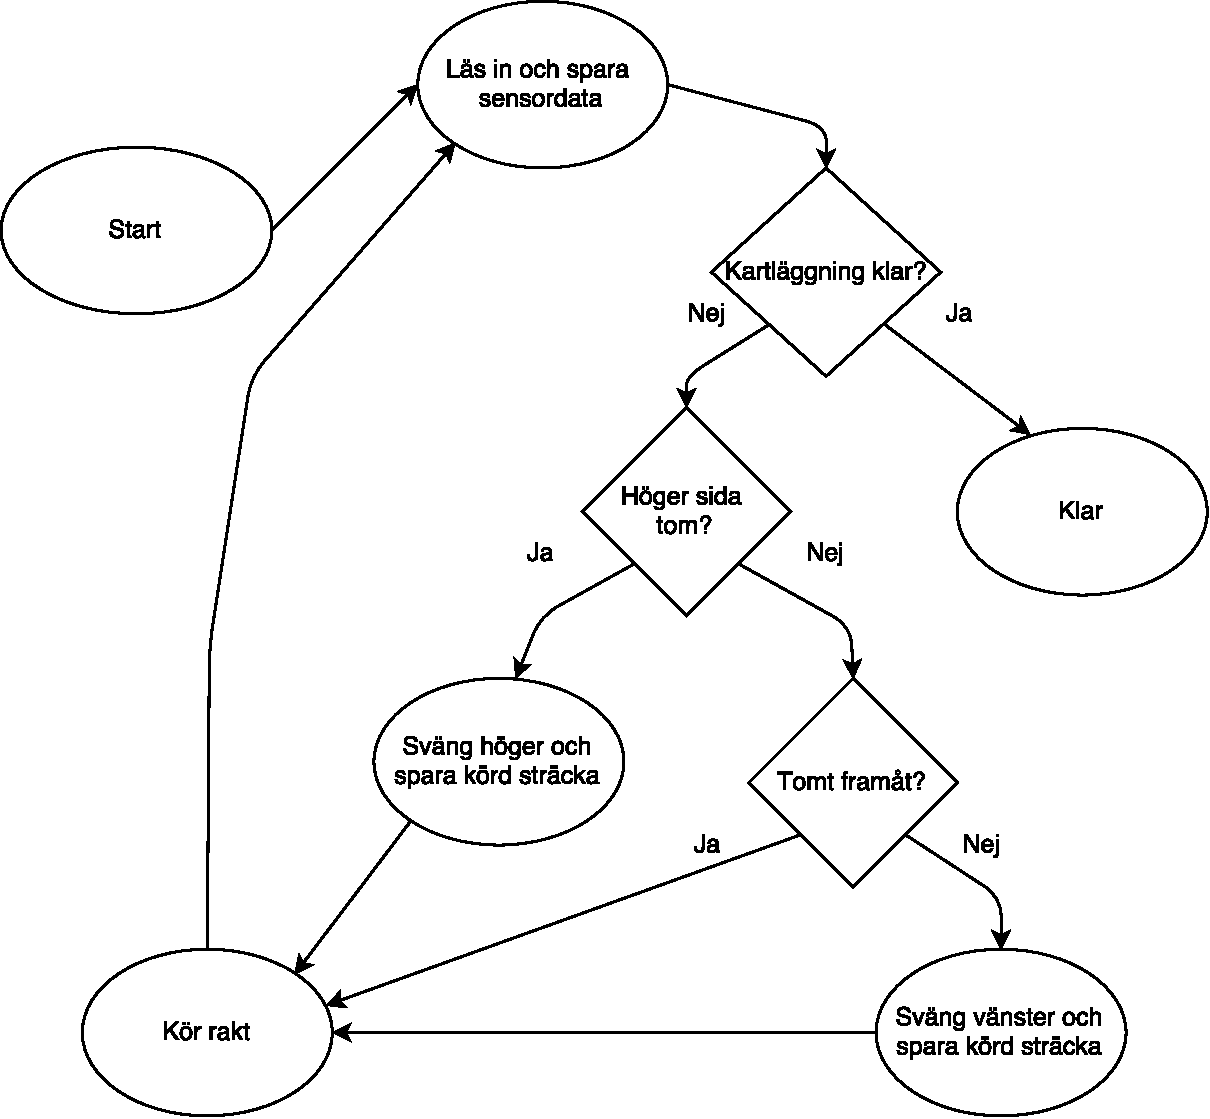
\includegraphics[scale=0.6]{navigering_flowchart}
\caption{Flödesdiagram för navigering.}
\label{fig:navigering_flowchart}
\end{figure}
I figur~\ref{fig:navigering_flowchart} ses en illustration över algoritmen för att följa en vägg på höger sida om roboten. Eftersom roboten börjar vid en vägg enligt tävlingsspecifikationen så kan den följa den direkt. När den sedan kartlagt den yttre väggen söker den efter köksön och faller sedan in i samma algoritm igen.


\begin{figure}[H]
\centering
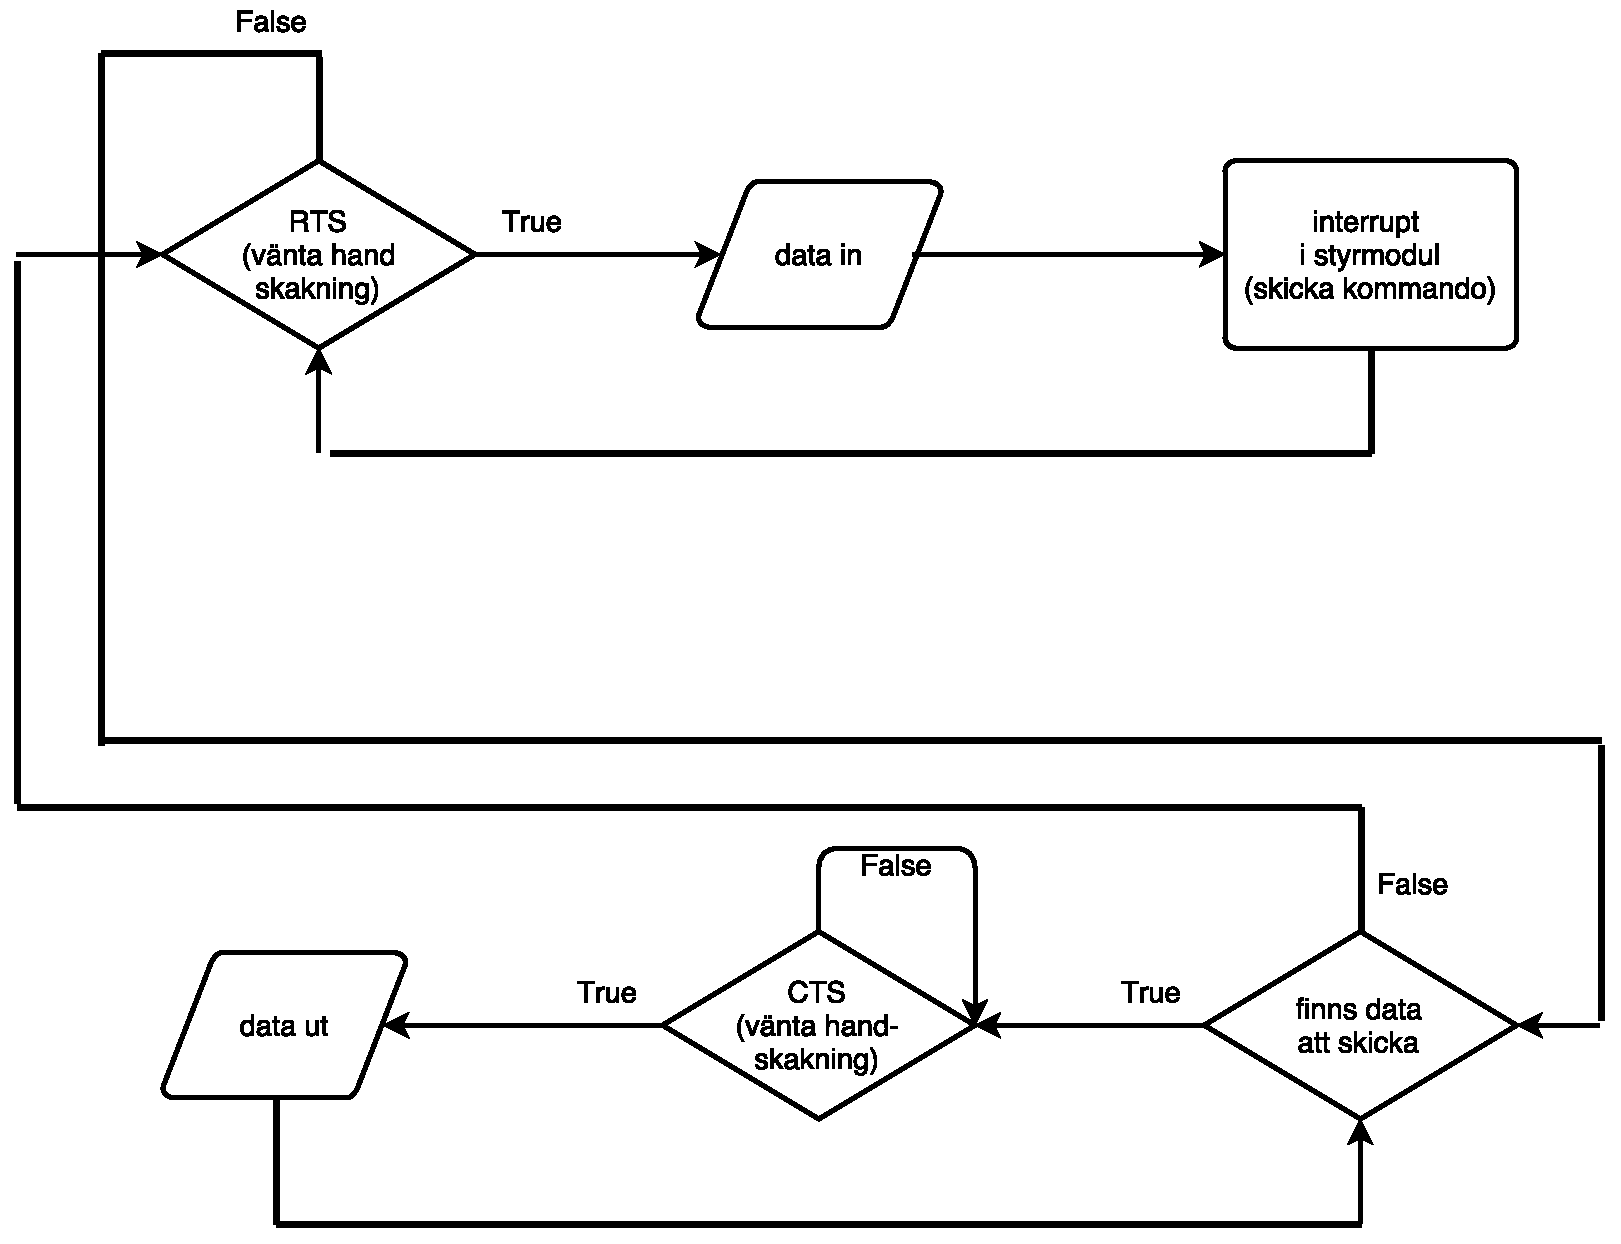
\includegraphics[scale=0.45]{Bluetooth_kommunikation_i_robot}
\caption{Flödesschema över Bluetooth-kommunikationen i huvudenheten.}
\label{fig:Bluetooth_kommunikation_i_robot}
\end{figure}

Flödesschemat i figur~\ref{fig:Bluetooth_kommunikation_i_robot} visar hur kommunikationen med mjukvaruklienten sköts ifrån huvudenheten. Då huvudenheten kommer att agera master i Bluetooth-kommunikationen (se avsnitt 4.2.2) krävs det att huvudenheten hanterar de signaler som sker vid kommunikation med Bluetooth. Figuren visar även hur en handskakning först måste inväntas innan en anslutning kan upprättas och data skickas eller tas emot. RTS och CTS-signalerna är som beskrivit handskakningssignaler. När (styrkommando-)data kommer till huvudenheten från mjukvaruklienten skickas denna vidare till styrenheten och orsakar ett interrupt. Om det ej finns någon data att ta emot kollas istället om det finns data att skicka. 


% Saxat från checklista:
%   Behövs det några speciella algoritmer för att lösa uppgiften?
%   Behövs det några större datastrukturer som kräver mycket minne?
%   Vilka avbrott ska användas och vad ska avbrottsrutinerna utföra?
%   Vilka funktioner ska utföras i en ”huvud-loop”?
%   Hur samverkar avbrottsrutinerna med huvudloopen?

\clearpage

\subsection{Sensorenhet}
% Se kommentarer för huvudenhet
Sensorenheten kommer ha i uppgift att läsa in värden från sensorerna som finns placerade på roboten och rapportera detta till huvudenheten. Detta kommer att ske genom att processorn pollar information från varje sensor i iterationer och sparar undan i minnet. Huvudenheten kommer att fråga sensorenheten efter nya mätdata och sensorenheten kommer då att kommunicera detta över I2C bussen.

\subsubsection{Delsystemets funktion}

Sensorenheten kommer att bestå av en ATMega 1284 processor som kommer att ha sensorer kopplad till sig. Processorn kommer att läsa av mätdata från sensorerna kontinuerligt och sparar undan dessa i minnet. Vid förfrågan av huvudenheten kommer processorn att leverera mätdata via huvudbussen. 
\newline\newline
Sensorenheten kommer att ha en lasersensor som läser av avståndet framåt. Denna sensor leverar mätvärden över gränsnitten PWM och I2C. Sensorenheten kommer att läsa av lasersensorn med PWM och omvandla till ett avstånd som kan sparas och levereras till huvudenheten vid förfrågan. I ett senare skede i projektet när vi har en fungerande robot så kommer vi att välja att gå över till en mer avancerad variant av kartläggning och då kommer lasersensorn att rotera runt roboten. Detta för att kunna använda oss utav metoden raycasting när rummet ska kartläggas.
\newline\newline
Sensorenheten kommer att ha två stycken IR-sensorer som ska läsa avstånd i sidan. Dessa sensorer levererar analoga värden och måste omvandlas till digitala värden. En tabell över värden kontra avstånd måste skapas för att kunna leverera exakta avstånd till huvudenheten vid förfrågan. 
\newline\newline
Sensorenheten kommer att ha en knapp som låter roboten växla mellan manuellt- och autonomt- läge.
\newline\newline
I det senare skedet av projektet när den avancerade kartläggningen kommer att användas så kommer roboten att använda sig av ett gyroskop för att hålla koll på hur mycket lasersensorn har roterat. Detta för att roboten ska veta vinkeln som lasern har rört sig under de olika mätpunkterna som ges.
\newline\newline
En accelerometer och gyroskop kommer att sitta på roboten för att kunna sköta reglering av roboten, hålla koll på hur långt roboten har åkt samt användas för att kunna korrigera de vinkelfel som blir om roboten roterar samtidgt som lasern roterar.

\subsubsection{Kopplingsschema}

\subsubsection{Komponenter}

\begin{table}[H]
  \centering
  \begin{tabular}{ | c | c | c | c |}
    \hline
    \textbf{Komponent} & \textbf{Antal} \\
    \hline
    ATMega 1284 & 1 \\
    \hline
    LIDAR-Lite v2 & 1 \\
    \hline
    Knapp & 1 \\
    \hline
    GP2Y0A21 IR-Sensor & 2 \\
    \hline
    MLX90609 Gyro & 1 \\
    \hline
    MPU6050 Accelerometer + Gyro & 1 \\
    \hline
  \end{tabular}
  \caption{ Tabell över de komponenter som sensorenheten består av. }
\end{table}

\subsubsection{Resurser}
% Rada upp tillgängliga portar på mikroprocessorn samt hur många som krävs
% Motivera val av mikroprocessor med uppskattning av de resurser som krävs (prestanda, minne, IO)

\begin{table}[H]
  \centering
  \begin{tabular}{ | c | c | c | c |}
    \hline
    \textbf{Port} & \textbf{Antal} & \textbf{Krävs} \\
    \hline
    SDA & 1 & 1 \\
    \hline
    SCL & 1 & 1 \\
    \hline
    IO & 32 & 2 \\
    \hline
    PCINT & 31 & 2 \\
    \hline
    OC & 8 & 2 \\
    \hline
    A/D & 8 & 2 \\
    \hline
    MISO & 1 & 1 \\
    \hline
    MOSI & 1 & 1 \\
    \hline
    SCK & 1 & 1 \\
    \hline
    SS & 1 & 1 \\
    \hline
    RXD & 2 & 1 \\
    \hline
    TXD & 2 & 1 \\
    \hline
    XCK & 2 & 1 \\
    \hline
  \end{tabular}
  \caption{Tabell över tillgängliga portar på processorn.}
\end{table}

En ATMega1284 måste användas i sensorenheten då accelerometer och gyroskopet använder sig av grännsnittet SPI för att kommunicera med omvärlden. Då det endast är ATMega1284 som har 2 eller fler SPI ingångar tvingas vi till att använda just denna.

\subsubsection{Programflöde}

\begin{figure}[H]
\centering
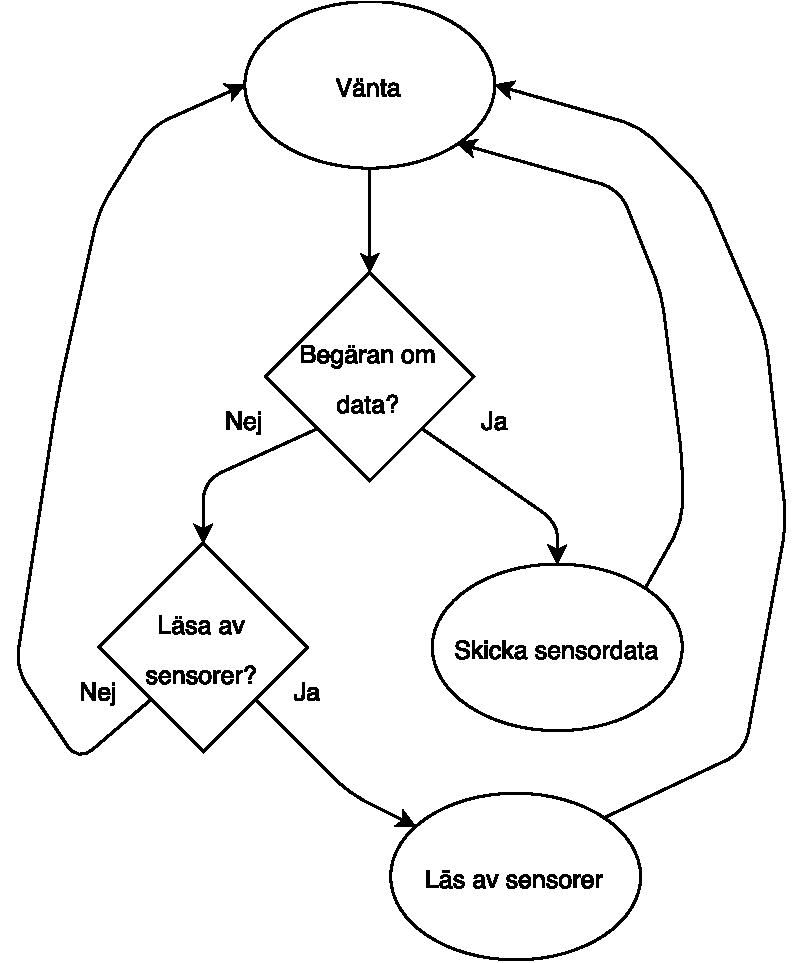
\includegraphics[scale=0.6]{sensorenhet_flowchart}
\caption{Ett flödesdiagram över sensorenhetens tillstånd}
\label{fig:sensorenhet_flowchart}
\end{figure}
Sensorenheten kan befinna sig i ett av tre lägen (se figur~\ref{fig:sensorenhet_flowchart}). Den läser antingen av sensordata, skickar sensordata, eller så befinner den sig i vänteläge. Sensorenheten kommer inte att ta några egna beslut om när den ska  skicka sensordata utan är helt beroende av att få kommando från huvudenheten för att skicka sensordata. Sensorenhetens huvudloop kommer att följa strukturen i flödesdiagramet i figur~\ref{fig:sensorenhet_flowchart}. Standardläget för sensorenheten kommer att vara vänteläget där den befinner sig tills en av två saker händer. Antingen kommer en instruktion ifrån huvudenheten som instruerar sensorenheten att skicka sensordata till huvudenheten. Då kommer datan att skickas via huvudbussen till huvudenheten, och sedan återgår sensorenheten till vänteläget. 
\newline\newline
Det andra som kan bryta sensorenhetens vänteläge är att den ska läsa in och spara sensordata. Sensorenheten kommer ha ett flertal sensorer kopplade till sig som ska läsas av så snart det är möjligt, men varje enskild sensor har en maximal inläsningstakt som inte kan överskridas. Det är alltså inte möjligt att läsa av varje sensor precis hela tiden, utan det är en viss väntetid mellan inläsningarna. Detta kommer sensorenheten att ha koll på, och så fort en sensor är redo för inläsning kommer värdet att läsas in, i den mån det behövs filtreras och/eller omvandlas datan, och sparas sedan för att kunna skickas iväg till huvudenheten när den ber om det. 

\clearpage

\subsection{Styrenhet}
% Se kommentarer för huvudenhet
Styrenhetens uppgift är att kontrollera alla robotens fysiska rörelser med hjälp av servon, baserat på kommandon ifrån huvudenheten. Det är genom styrenhetens funktionalitet  som roboten kommer att kunna förflytta sig igenom rummet som ska kartläggas.
 
\subsubsection{Delsystemets funktion}
Styrenheten kommer att bestå av en ATMega 1284 processor som kommer att ha servon kopplade till sig. Ifrån huvudenheten kommer kommandon som säger åt roboten att exempelvis åka framåt eller rotera. Kommandon som kommer ifrån huvudenheten översätts till signaler som skickas ut till styrenhetens servon för att kontrollera robotens rörelser. Processorn ska även ta emot och skicka vidare styrdata ifrån servona den har kopplade till sig.
\newline\newline
Fyra servon med hjul fastsatta på dem sitter ihopkopplade på ett chassi. De sitter två servon på varsin sida av chassit på samma sätt som hjulen sitter på en bil. Dessa servon är parkopplade, det vill säga att de två servona på vänstra sidan sitter ihop, och de på högra sidan sitter ihop. Höger och vänster hjulpar styrs alltså oberoende av varandra, och genom att skicka olika signaler till de båda hjulparen ska roboten kunna åka framåt och bakåt samt rotera. Hela konstruktionen heter Terminator och ses som en enskild enhet.
\newline\newline
Styrenheten kommer ha ytterligare ett servo kopplat till sig. På detta servo kommer två sensorer från sensorenheten att vara kopplade, en lasersensor samt ett gyro. I projektets första stadie kommer detta servo inte fylla någon funktion då lasersensorn monterad på den endast ska peka i en riktning, men i ett senare stadie kommer servot att rotera dessa två sensorer för att lättare och snabbare kunna detektera ouppsökta områden och kartlägga rummet.


\subsubsection{Kopplingsschema}

\subsubsection{Komponenter}

\begin{table}[H]
  \centering
  \begin{tabular}{ | c | c |}
    \hline
    \textbf{Komponent} & \textbf{Antal} \\
    \hline
    ATMega 1284 & 1 \\
    \hline
    Terminator (bas för fyrhjulingsrobot) & 1 \\
    \hline
    AX12-A Servo & 1 \\
    \hline

  \end{tabular}
\end{table}

\subsubsection{Resurser}
\begin{table}[H]
  \centering
  \begin{tabular}{ | c | c | c | c |}
    \hline
    \textbf{Port} & \textbf{Antal} & \textbf{Krävs} \\
    \hline
    SDA & 1 & 1 \\
    \hline
    SCL & 1 & 1 \\
    \hline
    IO & 32 & 7 \\
    \hline
  \end{tabular}
  \caption{Tabell över tillgängliga portar på processorn.}
\end{table}

Omvandlingen av kommandon från huvudenheten och utskickning av signaler till servona samt omhändertagandet och vidarebefodrandet av styrdata från servona till huvudenheten uppskattas ej kräva mer prestanda eller minne än styrenhetens ATMega 1284 processor klarar av.
\newline\newline
Den maximala hastigheten som sensordata kan läsas in i är begränsad av sensorernas rapporteringsfrekvens som är betydligt långsammare än en ATmega 1284:s klockfrekvens, därför lönar det sig inte med en snabbare processor för sensorenhetens syfte. Det i princip enda minnet sensorenheten kommer använda sig av är för temporärlagring av alla sensorers data, vilket kommer hålla sig runt 20 bytes. Utöver sensorinläsningen kommer enheten svara på kommandon över huvudbussen som inte heller kräver några höga hastigheter eller minneskrav. En mer ingående motivering till dessa resurskrav finns i avsnitt~\ref{sec:samplingsfrekvens}.

\subsubsection{Programflöde}

\begin{figure}[H]
\centering
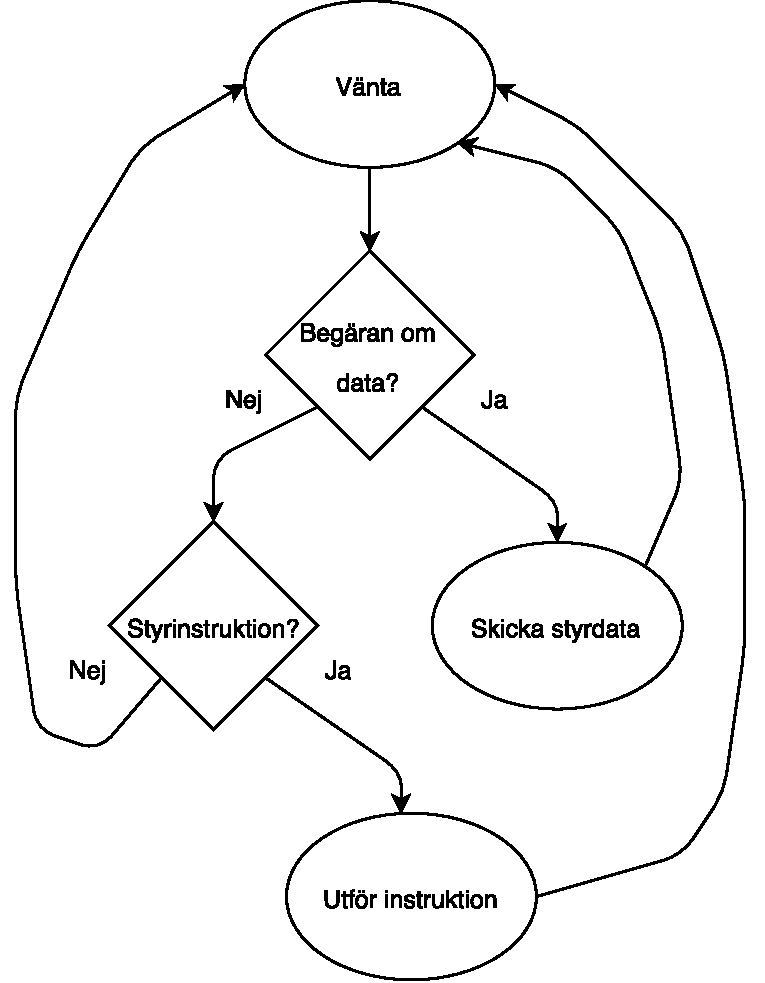
\includegraphics[scale=0.6]{styrenhet_flowchart}
\caption{Ett flödesschema över styrenhetens tillstånd}
\label{fig:styrenhet_flowchart}
\end{figure}
Styrenheten har tre olika tillstånd den kan befinna sig i. Antingen skickar den styrdata, utför en instruktion eller så befinner den sig i vänteläge. Figur~\ref{fig:styrenhet_flowchart} visar visuellt hur styrenheten rör sig mellan dessa tre tillstånd. Dess standardtillstånd är vänteläget som den befinner sig i tills den fått en instruktion ifrån huvudenheten. Till skillnad från sensorenheten som läser av sina sensorer utan något kommando från huvudenheten kommer styrenheten inte att göra något utan att ha fått en instruktion ifrån huvudenheten att utföra. I vänteläget kommer styrenheten invänta instruktioner från huvudenheten, av vilket det finns två olika typer. Antingen är det en begäran om data, och isåfall kommer styrenheten att skicka tidigare sparad styrdata till huvudenheten. Annars är det en styrinstruktion (som exempelvis att åka framåt, bakåt eller svänga), i vilket fall styrenheten kommer att omvandla den instruktionen till signaler att skicka till de servon som är kopplade till processorn. I det här tillståndet kommer även styrdata insamlat från servona sparas för att kunna skickas till huvudenheten när det kommer en förfrågan om det.
\clearpage

\subsection{Presentationsenhet}
% Se kommentarer för huvudenhet
Presentationsenheten är del av mjukvaruklienten och har till uppgift att presentera mät-/ och styrdata samt presentera kartdatan i form av en grafisk karta. Informationen ska presenteras genom mjukvaruklientens GUI och uppdateras kontinuerligt när ny data mottages från robotens huvudenhet. 

\subsubsection{Delsystemets funktion}
Presentationsenhten får sin data från mjukvaruklientens kommunikation med robotens huvudenhet. Denna kommunikation sker via Bluetooth (se avsnitt 4.2). När datan aländer till presentationsenheten sorteras den utifrån medföljande ID, enligt kommunikationsprotokollet. De tre typerna av data är kart-, mät- och styrdata. Mät- och styrdatan kommer ursprungligen från robotens sensorer, gyroskop och accelerometrar. Kartdatan genereras av robotens huvudenhet och är underlaget för den grafiska utritningen av kartan i presentationsenheten. Formatet på kartdatan kommer vara sådant att den utgår från robotens startposition - vilket blir origo i koordinatsystemet - och i någon form sparar hörn som noder. 

\subsubsection{Blockschema}
% Övergripande schema för systemets stuktur
\begin{figure}[H]
%\centering
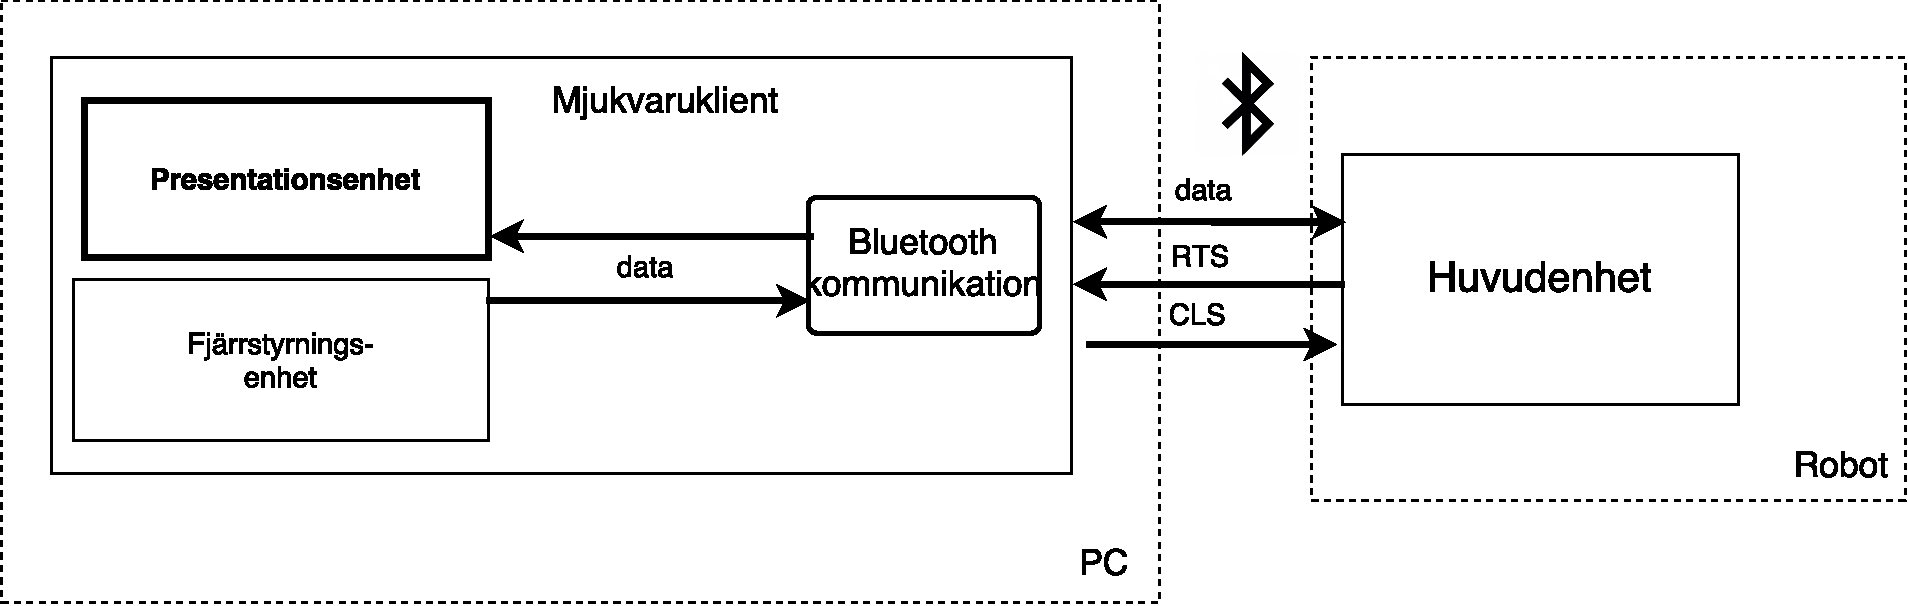
\includegraphics[scale=0.37]{Oversikt_presentationsenhet2}
\caption{Presentationsenheten i omgivning}
\label{fig:Oversikt_presentationsenhet2}
\end{figure}
Ovanstående figur~\ref{fig:Oversikt_presentationsenhet2} visar presentationsenheten i sin omgivning. Den kommunicerar via mjukvaruklientens Bluetooth-förbindelse med robotens huvudenhet. RTS- och CTS-signalerna används för handskakning mellan enheterna, dvs. styr vem som skickar respektive tar emot data.  

\subsubsection{Komponenter}
Mjukvaruklienten och därmed presentationsenheten kräver en bärbar dator med Bluetooth. 

\subsubsection{Resurser}
Presentationen och behandlingen av datan som presentationsenhet mottager uppskattas ej kräva mer minne eller prestanda än vad den tillhandahållna bärbara datorn klarar av.

\subsubsection{Programflöde}
\begin{figure}[H]
\centering 
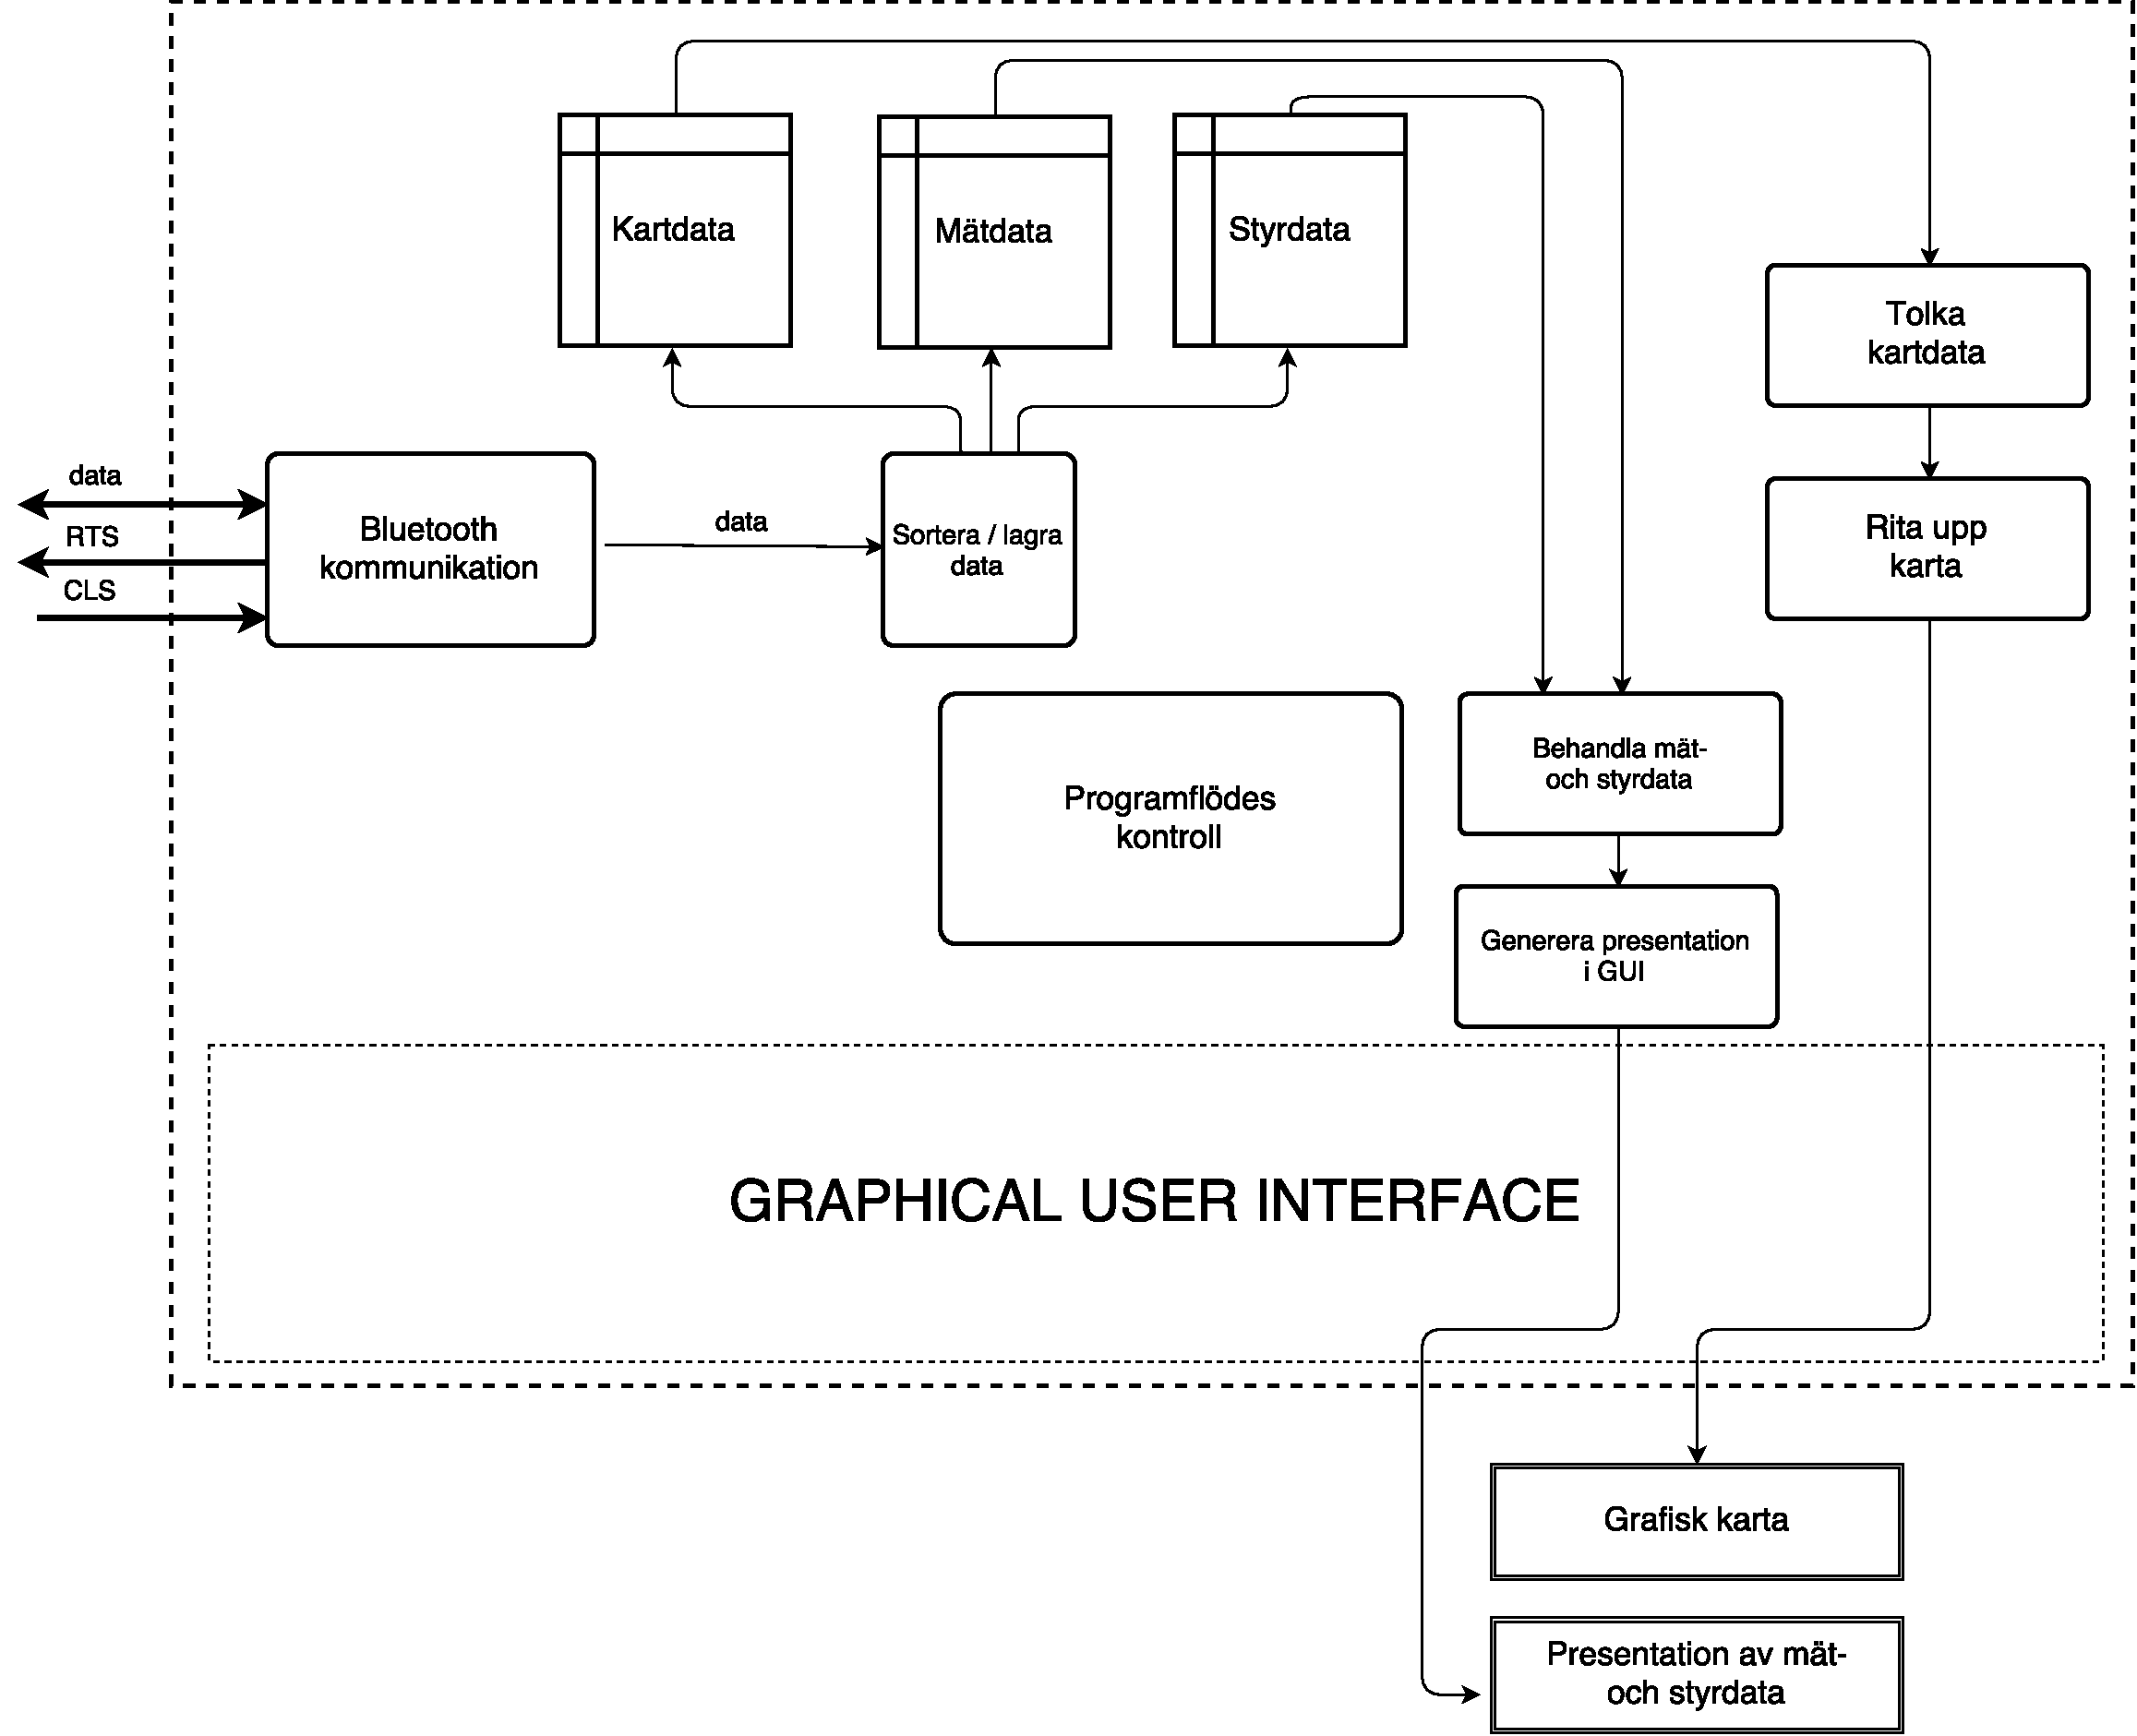
\includegraphics[scale=0.3]{Presentationsenhet}
\caption{Flödesschema över presentationsenheten}
\label{fig:Presentationsenhet}
\end{figure}
Som man kan se i ovanstående figur~\ref{fig:Presentationsenhet} måste den inkommande datan sorteras utifrån medföljande ID och lagras i lämpliga datastrukturer. Datastrukturerna bör kunna sortera sin data utifrån tid, för mät- och styrdata, samt tid och position för kartdata. Tiden behöver registreras för att mjukvaruklienten ska kunna begära rätt data från huvudenheten utifrån den senaste datan mottagen. Detta är även användbart om vi behöver återhämta information från robotens huvudenhet vid eventuell krasch och förlust av data i mjukvaruklienten (observera att denna funktion är klassificerad med prioriteringsnivå 2 i \textit{Kravspecifikationen}). Programflödet i presentationsenheten kommer styras centralt i mjukvaruklienten, som har ansvar för att växla mellan behandling av I/O (dvs. växla mellan att låta presentations- respektive fjärrstyrningsenhet arbeta). 

\clearpage

\subsection{Fjärrstyrningsenhet}
% Se kommentarer för huvudenhet
Fjärrstyrningsenheten är liksom presentationsenheten en del av mjukvaruklienten. Fjärrstyrningsenhetens huvudsakliga uppgift är att låta en användare skicka kommandon via mjukvaruklienten till roboten, med syfte att kunna kontrollera robotens fysiska position manuellt. I ett senare skede av projektets utveckling är det även tänkt att det ska gå att växla mellan robotens autonoma och manuella läge igenom fjärrstyrningsenheten, men det är en funktion som är lägre prioriterad än de andra.

\subsubsection{Delsystemets funktion}
Fjärrstyrningsenheten tar emot input av en användare som kommer genom mjukvaruklienten. Användarinput hämtas genom interaktion med mjukvaruklienten via datorn som mjukvaruklienten används på. Den informationen packeteras och skickas sedan vidare till robotens huvudenhet via Bluetooth (se avsnitt 4.2). Väl i huvudenheten sköter roboten så att kommandona skickas vidare till styrenheten som i sin tur gör att roboten förflyttar, så fjärrstyrningsenhetens enda jobb är att förmedla användarens input till huvudenheten.


\subsubsection{Blockschema}
% Övergripande schema för systemets stuktur
\begin{figure}[H]
\centering 
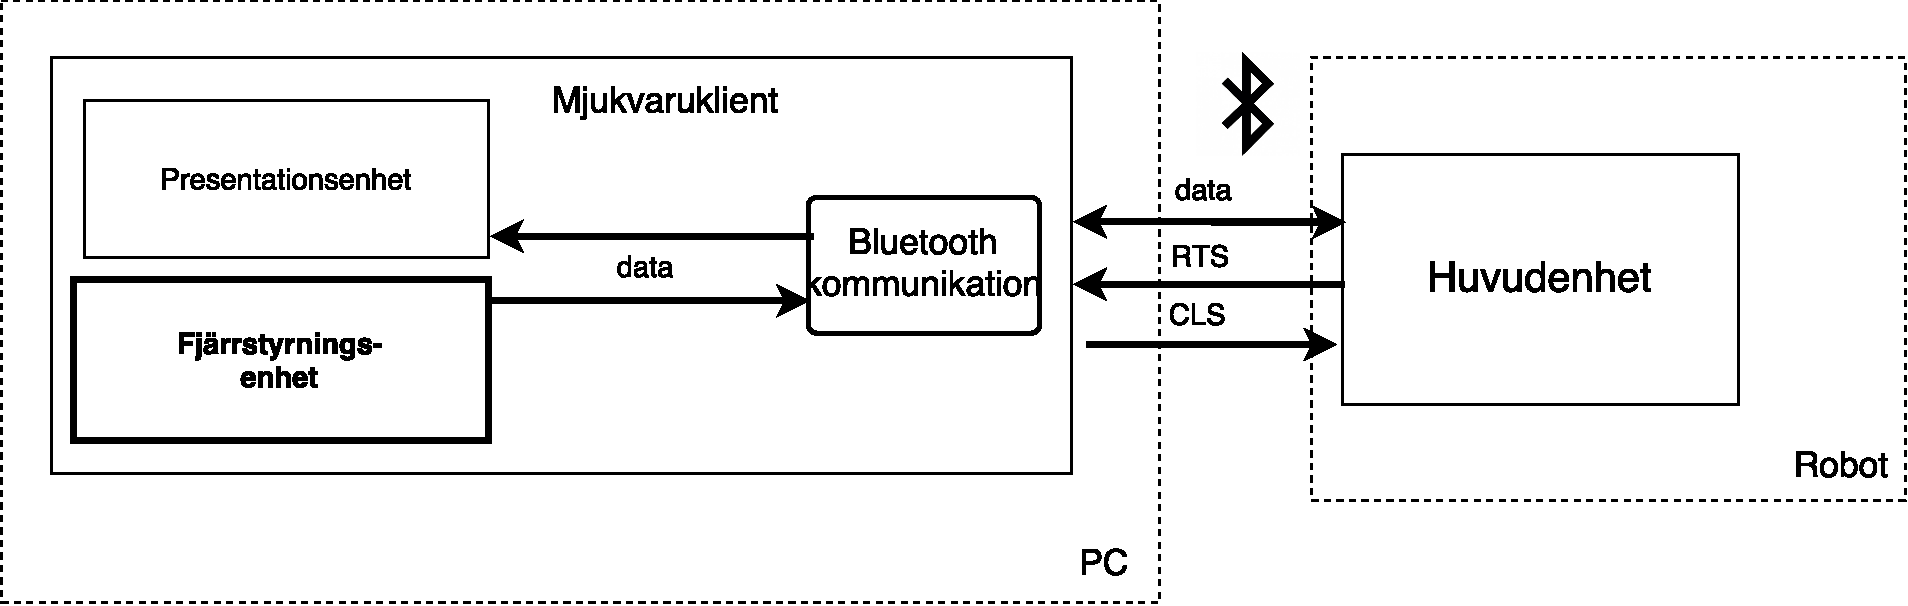
\includegraphics[scale=0.37]{Oversikt_fjarrstyrenhet}
\caption{Fjärrstyrningsenheten i omgivning}
\label{fig:Oversikt_fjarrstyrenhet}
\end{figure}
Ovanstående figur~\ref{fig:Oversikt_fjarrstyrenhet} visar fjärrstyrningsenheten i sin omgivning. Den kommunicerar via mjukvaruklientens Bluetooth-förbindelse med robotens huvudenhet. RTS- och CTS-signalerna används för handskakning mellan enheterna, dvs. styr vem som skickar respektive tar emot data.  

\subsubsection{Komponenter}
Fjärrstyrningsenheten kräver en dator med Bluetooth som kan köra mjukvaruklienten, samt tangentbord och mus/touchpad för interaktion med klienten. 

\subsubsection{Resurser}
Funktionaliteten för att ta emot användarinput och skicka iväg den via Bluetooth uppskattas ej kräva mer minne eller prestanda än vad den tillhandahållna datorn klarar av.

\subsubsection{Programflöde}
\begin{figure}[H]
\centering 
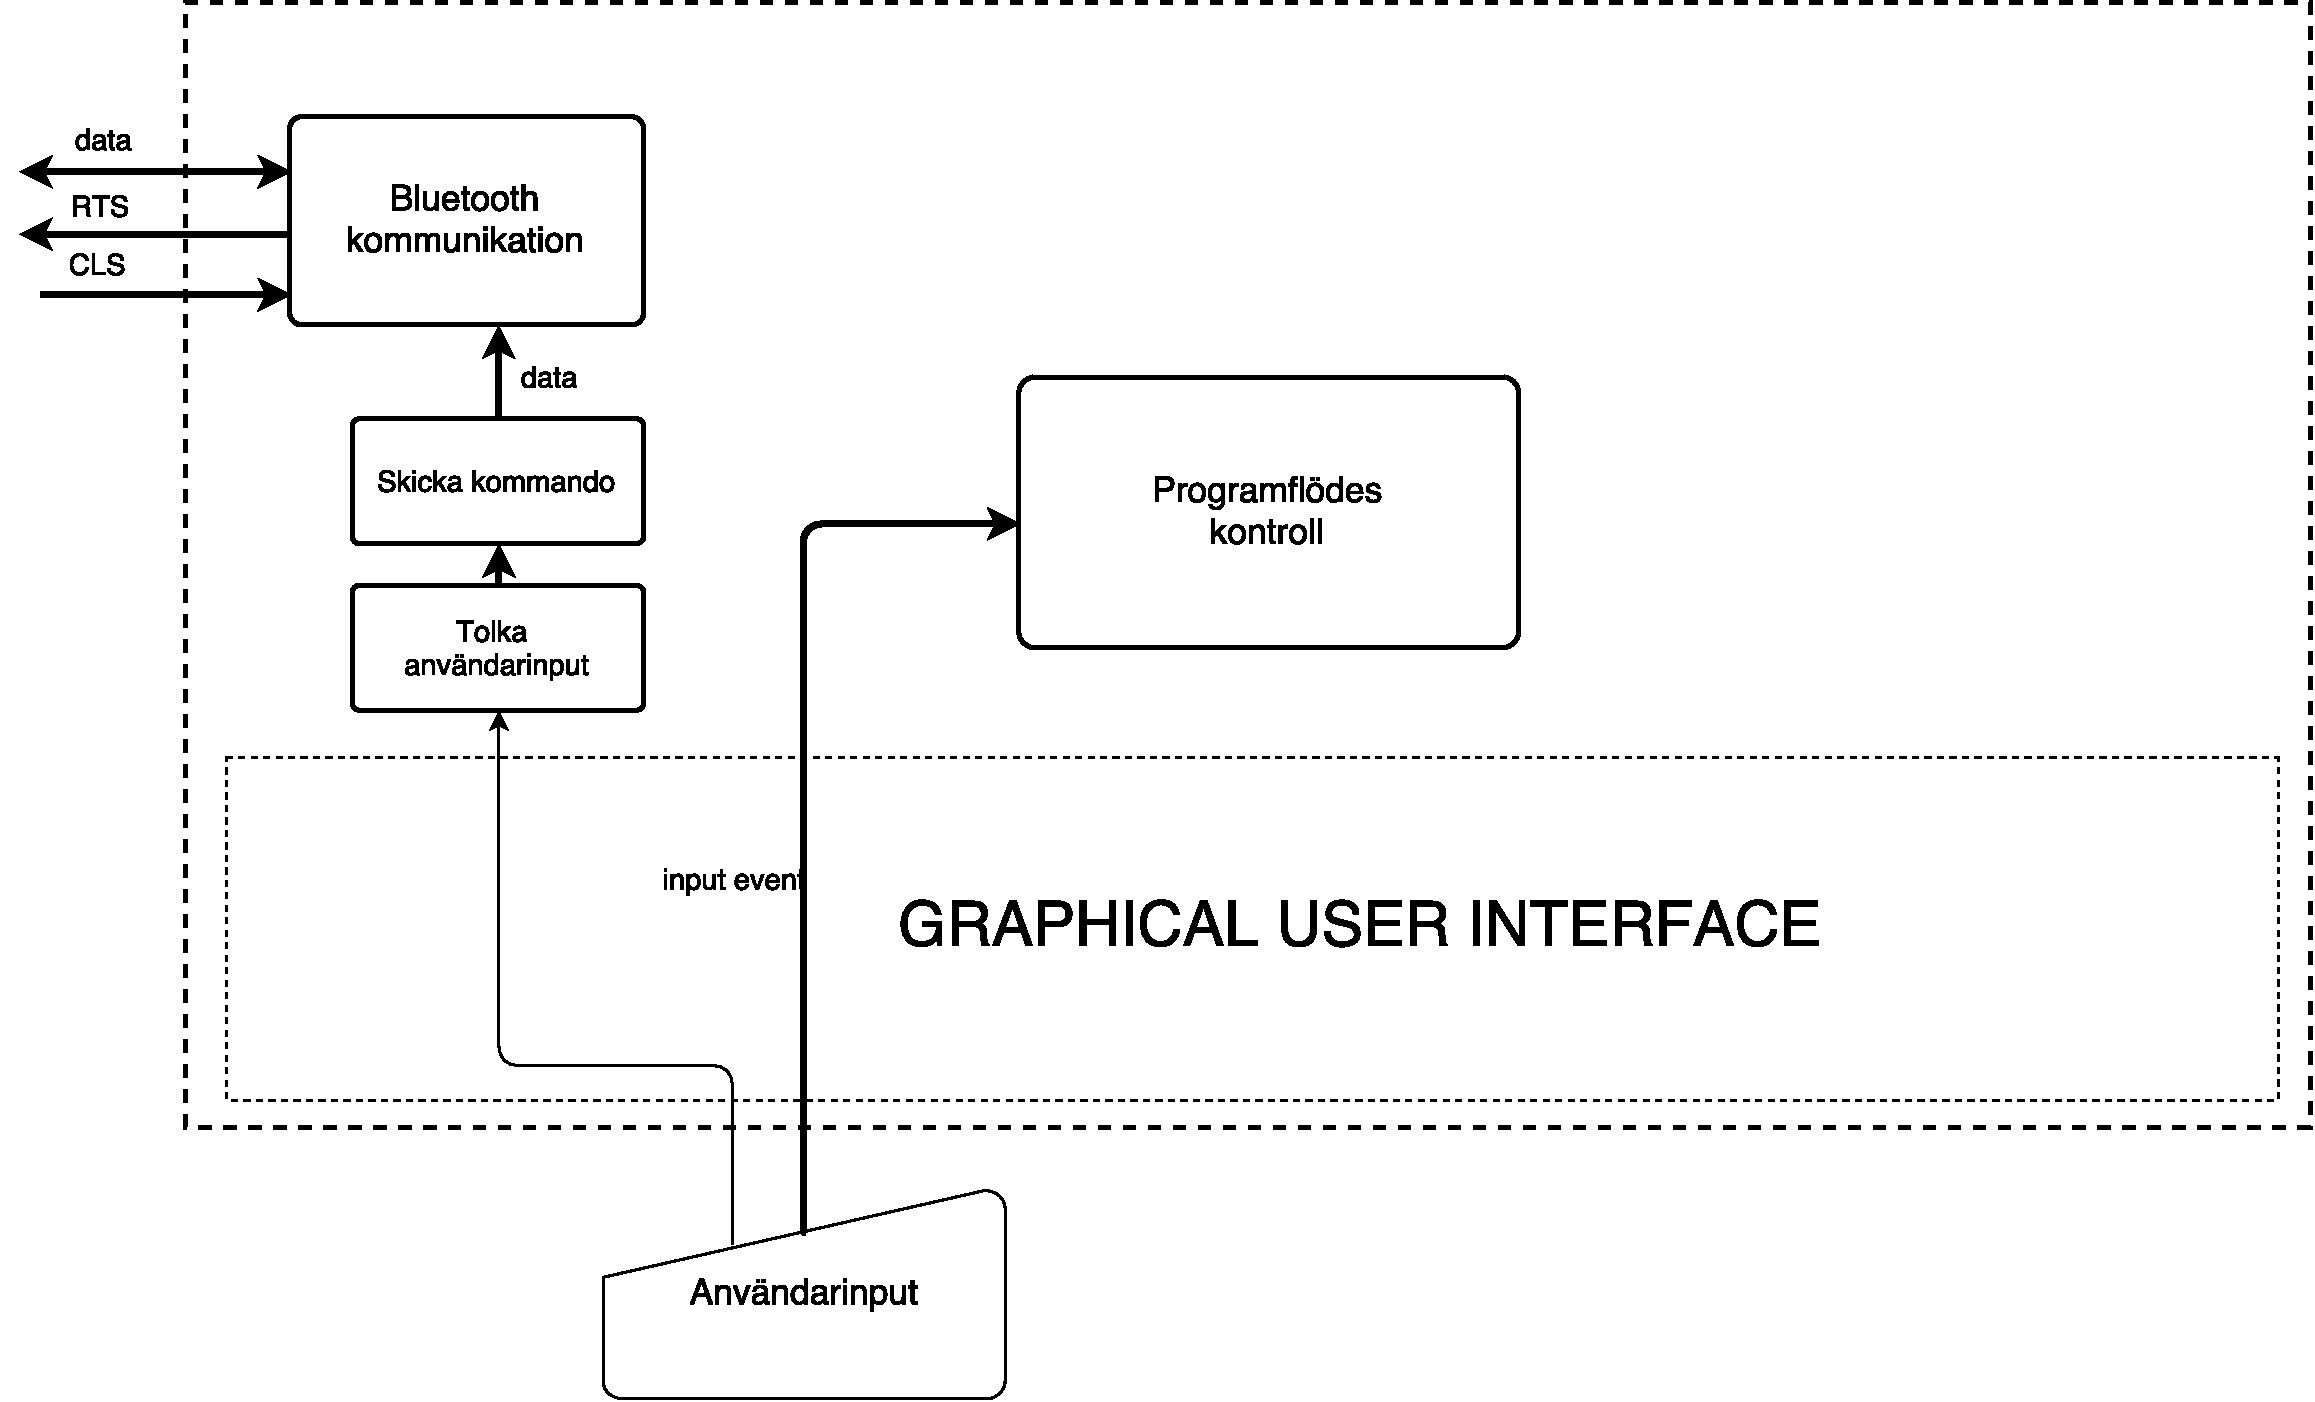
\includegraphics[scale=0.3]{Fjarrstyrningsenhet_flowchart2}
\caption{Flödesschema över fjärrstyrningssenheten}
\label{fig:Fjarrstyrningsenhet_flowchart2}
\end{figure}
Som visas i ovanstånde figur~\ref{fig:Fjarrstyrningsenhet_flowchart2} ger användaren input till fjärrstyrningsenheten. Inputet kommer orsaka någon form av input-event som påverkar programflödeskontrollen i mjukvaruklienten. Detta input tolkas sedan för att motsvara rätt kommando som sedan ska skickas via Bluetooth-anslutningen till robotens huvudenhet (för en lista över kommandon, se \textit{Kravspecifikationen}).

\clearpage

\section{Kommunikation mellan delsystem}
Kommunikation mellan systemets enheter kommer att ske över både en fysisk huvudbuss samt en trådlös Bluetooth-uppkoppling till presentations- och fjärrstyrningsenheten. Under teknikernas basprotokoll kommer de båda kommunikationsmedierna använda sig av samma protokoll. Detta är dels för att kunna återanvända samma lösning vilket förenklar utvecklingsprocessen, dels för att förenkla hanteringen av kommunikationen i huvudenheten. Genom att använda samma protokoll för kommunikation över Bluetooth och huvudbussen kan kommunikationen hanteras på ett och samma ställe inom huvudenheten, istället för att behöva dela upp kommunikationshanteringen. Protokollet specificeras senare i projektets skede för att kunna testa dess funktion innan det bestäms.

% Kort inledning. Nämn att huvudbuss och Bluetooth använder ett "underliggande" protokoll (under I2C/Bluetooth) som specificeras under projektets gång

\subsection{Huvudbuss}
Systemets moduler på roboten kommer vara sammankopplade med en I2C-buss (även kallat Two-Wire-Interface) där huvudenheten skickar och tar emot kommandon från sensor- och styrenheten. Trots att gränssnittet stödjer kommunikation mellan bussens alla enheter kommer endast kommunikation direkt till och från huvudenheten att implementeras för att kunna hålla systemets beroenden så pass frikopplade som möjligt.

\subsubsection{Uppbyggnad}
Bussen består så som dess alternativa namn antyder av ett två-trådat gränssnitt och stödjer upp till 128 enheter. De två trådarna är SDA och SCL där SDA överför data medan SCL styr med vilken frekvens detta sker. SDA kommer skrivas på av bussens alla inkopplade enheter och behöver kopplas in till ett pull-up-motstånd för att inte flyta. Uppbyggnaden av bussen och dess master-slave förhållande kan ses i figur~\ref{fig:huvudbuss_masterslave}.

\subsubsection{Master-slave roller}
\begin{figure}[H]
\centering 
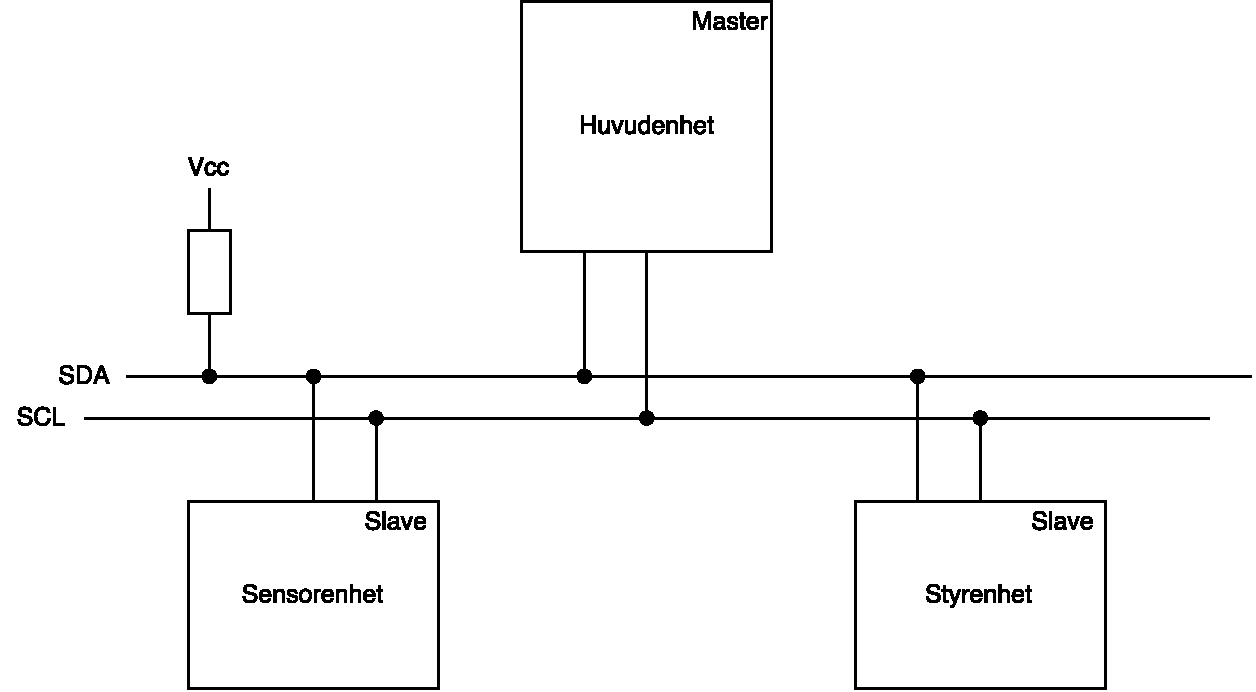
\includegraphics[scale=0.56]{Huvudbuss}
\caption{Huvudbussens uppbyggnad och master-slave förhållande}
\label{fig:huvudbuss_masterslave}
\end{figure}

I2C har två olika implementationer: multimaster och master-slave, som båda skiljer en del till implementationen. Multimaster är svårare att implementera då flera olika mikroprocessorer behöver styra bussens klock-pin. Detta system kommer använda sig av den enklare master-slave-implementationen för att kunna lägga tid på mer användbara funktioner samt eftersom Raspberry Pi:s egna I2C-implementationen endast stödjer just det läget. Huvudenheten kommer att agera master i konfigurationen för huvudbussen och generera en klocka på SCL-pinnen från det att bussens startvillkor inträffat till dess att stoppvillkoret är uppfyllt. Bussens start- och stoppvillkor är designade så att de inte kan inträffa samtidigt som man överför riktig data. Resten av enheterna agerar slavar, se figur~\ref{fig:huvudbuss_masterslave}.

% Beskriv huvudbussen. Vad använder vi för teknik? Hur ser master/slave-förhållande ut?
% Använd med fördel \subsubsection

\subsection{Bluetooth}
% Beskriv Bluetooth. Vad använder vi för teknik? Hur ser master/slave-förhållande ut?
% Använd med fördel \subsubsection
Datorn som mjukvaruklienten är installerad behöver kunna kommunicera roboten för att det ska gå att rita upp kartan samt kunna fjärrstyra roboten ifrån datorn. Då det skulle vara opraktiskt att ha en sladd mellan datorn och roboten kommer kommunikationen istället ske trådlöst via Bluetooth. 

\subsubsection{Handskakning}
\begin{figure}[H]
\centering 
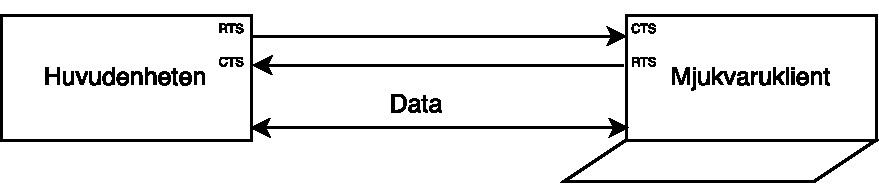
\includegraphics[scale=0.8]{Kommunikation_Bluetooth}
\caption{Bluetooth mellan huvudenheten och mjukvaruklienten}
\label{fig:Kommunikation_Bluetooth}
\end{figure}

Som figur~\ref{fig:Kommunikation_Bluetooth} visar går det ett antal signaler mellan huvudenheten och mjukvaruklienten. Till en början finns två signaler som går från respektive Bluetoothmoduls RTS (\textit{Request to send}) till den andra enhetens CTS (\textit{Clear to send}) som används för handskakning mellan de båda Bluetoothenheterna. Handskakningen krävs för att upprätta en förbindelse mellan de två modulerna för vidare kommunikation. När en förbindelse väl har upprättats kommer de att automatiskt återansluta till varandra om de skulle tappa kontakten. Om datorn exempelvis skulle föras längre ifrån roboten än räckvidden för Bluetoothanslutningen och sedan föras tillbaka igen skulle datorn och roboten känna igen att de varit anslutna till varandra med Bluetooth förut, och därefter automatiskt ansluta igen.
\newline\newline
När en anslutning väl är upprättad kan data skickas mellan de båda enheterna.

\subsubsection{Master-slave roller}
När Bluetooth-anslutningen väl är upprättad mellan roboten och datorn går det att skicka data mellan de två. Liksom med huvudbussen finns ett master-slave förhållande mellan de olika Bluetooth-modulerna. I det här fallet kommer huvudenhetens Bluetooth-modul agera master och datorn slave.

\subsection{Informationsflöde}
Tanken med hur informationen flödar mellan delsystemen är att den ska skickas som asynkrona så kallade kommandon eller paket. Genom att specificera detta kan informationsflödet implementeras med valfri asynkron buss eller kommunikationsmedie och det blir även möjligt att abstrahetera bort varifrån alla meddelanden kommer. I respektive delsystem kommer alla kommandon hanteras som event och vid behov även returnera data genom att skicka ett nytt asynkront kommando tillbaka som svar.

\subsubsection{Kommunikation med sensorenhet}
Den enda data som skickas från huvudenheten till sensorenheten är en förfrågan om att hämta mer data och på samma sätt är den enda data som skickas åt andra hållet den mätdata som sensorenheten för närvarande innehåller. Sensorenheten är inte ansvarig för att själv skicka denna data då huvudenheten enklare kan bestämma hur ofta data ska skickas. Med denna lösning blir sensorenhetens enda egna uppgift att läsa in data och spara det i dess minne.

\subsubsection{Kommunikation med styrenhet}
Precis som för sensorenheten kommer huvudenheten efterfråga data från styrenheten i form av styrdata. Utöver detta kommer kommandon för att styra enhetens ställdon skickas från huvudenheten med kommandon som t.ex. framåt, bakåt, stopp, rotera 90{\textdegree} höger, etc. Vissa av dessa kommandon kommer resultera i styrning som fortföljer tills ett annat kommando skickas medan andra har ett avslut (t.ex. rotering 90{\textdegree}). De kommandon som har ett avslut skickar ett svar tillbaka till huvudenheten när de genomförts.

\subsubsection{Kommunikation med mjukvaruklient}
Mellan huvudenheten och mjukvaruklienten kommer mycket av den data som redan skickas på huvudbussen skickas även där efter den ompaketerats.
\newline\newline
Den data som skickas från mjukvaruklienten är följande
\begin{itemize}
\item Förfrågan om all ny kartdata sedan en viss tidpunkt t
\item Kommandon för att styra roboten
\item Byte av exekveringsläge
\end{itemize}
\ \\
Den data som skickas till mjukvaruklienten är följande
\begin{itemize}
\item All ny kartdata sedan tidpunkt t
\item Kontinuerlig kartdata
\item Kontinuerlig mätdata
\item Kontinuerlig styrdata
\item Verifikation av kommandon
\end{itemize}
\ \\
Notera att all kontinuerlig data som skickas är begränsad av den samplingsfrekvens som beskrivs i avsnitt~\ref{sec:samplingsfrekvens}. Kontinuerlig kartdata kommer inte att skickas förrän mjukvaruklienten efterfrågat kartdata minst en gång.

\clearpage

\section{Implementationsstrategi}
Detta avsnitt ger en inblick i hur projektet ska utvecklas, testas, och vilka kritiska sektorer som finns, med huvudsyfte att ge utvecklarna tydliga riktlinjer att följa.

\subsection{Utvecklingsstrategi}
För att snabbare få ett demonstrerbart resultat kommer projektet utvecklas iterativt där aktiviteterna utgör sprinter till nästa milstolpe. Detta innebär att all funktionalitet som implementeras för en milstolpe kommer slutföras i en ensam, icke-parallell aktivitet. Att utveckla på det här sättet gör att vi tydligare kan se konkreta saker bli klara och verifiera deras funktionalitet tillsammans med deras beroenden, vilket beskrivs tydligare i avsnitt~\ref{sec:testbarhet}. Med denna utvecklingsstrategi följer även nackdelen att arbetet blir svårare att parallellisera och innebär också att arbetet per vecka behöver delas in i veckans två halvor för att alla aktiviteter ska hinna genomföras.
\newline\newline
Aktivitetsplanen för projektet är uppdelad i två delar där aktiviteterna är separerade i olika nivåer av komplexitet. Denna strukturering härstammar från projektets planering och ambitioner: det finns ambition och intresse för att implementera en mer avancerad lösning på kartläggningsproblemet roboten ska lösa, men risken är för stor att den algoritm gruppen har i åtanke inte alls kommer att fungera. För att fortfarande ha chans att skapa en robot med den mer avancerade funktionaliteten är aktiviteter för att realisera denna med i aktivitetsplanen men inplanerade i den andra delen. Den första delen bygger på en betydligt simplare och tidigare bevisat genomförbar algoritm och uppfyller alla krav med prioritet 1. De krav som har en prioritet 2 är också tillräckligt små för att implementera utan att inkludera den mer avancerade algoritmen fullt ut men är steg på vägen.

\subsection{Testfilosofi}
\subsubsection{Testbarhet}
\label{sec:testbarhet}
Ett krav för projektets alla aktiviteter är att de ska vara testbara från första början och inte får påbörjas förrän det kontinuerligt går att genomföra tester under utvecklingens gång tillsammans med den kringliggande miljö som krävs. Anledningen till detta härstammar från risken som uppstår om tid läggs på att undersöka funktionalitet och algoritmer som inte omedelbart kan verifieras. Det är onödigt att lägga många timmar på att ta fram en komplicerad algoritm som inte visar sig fungera i verkligheten. Genom att även kunna verifiera en aktivitets slutgiltiga funktionalitet kan den avslutas med säkerhet och bidra till att färre buggar introduceras.

\subsubsection{Enhetstester}
Ett viktigt moment i att verifiera en ensam funktions korrekthet är att skriva små enhetstester (eng. unit tests) som säkerställer att man får förväntad utdata givet en specifik indata. Dessa tester tjänar som syfte att minimera fel som sker i de många små byggstenar som bygger upp en komponent. Det går med fördel att skriva dessa tester utifrån komponentens design innan funktionaliteten implementeras eller genom att testa varandras kod i de fall man är ett flertal personer som arbetar på samma aktivitet. Alla enhetstester ska skrivas samtidigt som en aktivitet genomförs och används som underlag för att verifiera aktivitetens funktion och avslut.

\subsubsection{Systemtester}
När mjukvaran ska testas i verkliga scenarion kommer så kallade systemtester behöva genomföras. Detta kan inkludera att skicka data på huvudbussen eller reglera utmed en vägg. Eftersom många av de här testerna kräver att flera mikroprocessorer programmeras och ibland till och med att hela roboten förflyttas till en annan plats så medför det att dessa tester inte kan köras samtidigt. För att mitigera detta problem ska alla mer omfattande systemtester förvarnas om i god tid ifall de riskerar att krocka med andra tester. Systemtesterna är liksom enhetstesterna inräknat i varje aktivitet som kräver dessa. Notera att systemtesterna aldrig testar en bana i sitt kompletta utförande utan endast ett visst antal egenskaper, för att testa banspecifikationen se avsnitt~\ref{sec:bantester}.

\subsubsection{Bantester}
\label{sec:bantester}
När robotens tävlingsduglighet ska utvärderas kommer tester av banan i sitt kompletta utförande behövas. Det finns ett fåtal tillfällen avsatta för det här och robotens funktionalitet bör vara säkerställd innan testerna börjar för att slippa förlora den stora mängd tid som krävs för att bygga upp banan i korrekt format. Då mjukvaran för att kartlägga området är känslig för avvikelser i banans design är det viktigt att banan byggs nogrannt nog för att inte få följfel som härstammar från inexakta vinklar och mått. Under bantesterna ska hela gruppen samarbeta för att effektivisera testandet och snabbare kunna upptäcka varför eventuella fel framträder.

\subsection{Kritiska sektorer}
Under utvecklingens gång kommer det finnas kritiska moment som kan resultera i att tidigare genomfört arbete behöver modifieras eller blir fullkomligt invaliderat. Vissa kritiska moment kan undvikas i viss grad och nedan följer en uppradning av de mest kritiska momenten och hur de kan mitigeras.

\subsubsection{Kopplingsschema och virande}
Att vira upp alla kopplingar efter kopplingsschemat kan vara en pillig och tidskrävande aktivitet där missar kan leda till glappande kontakter som är svåra att felsöka. Aktivitetsplanen är stukturerad så att kopplingsschemat realiseras i olika steg vilket gör att det kommer uppstå olika lager av virtrådar allt eftersom projektet fortgår. Skulle ett av de tidigare stegen behöva korrigeras med andra kopplingar på grund av modifierat kopplingsschema kan mycket arbete alltså behöva göras om. För att undvika att sådana problem uppkommer bör kopplingsschemat kontrolleras och godkännas för varje del som ska kopplas innan virandet genomförs.

\subsubsection{Förändring av delade datastrukturer}
Ifall datastrukturer som används i fler än en enhet behöver modifieras i efterhand kan det kräva förändring i många olika delar av systemet. Det är svårt att förebygga det här för många av de strukturer som används annat än att granska och godkänna dem innan de implementeras. Vissa strukturer så som protokollet för huvudbussen och Bluetooth delas upp i olika lager så att de kan modifieras oberoende.

\subsubsection{Resurser}
Om projektet kör in i någon sorts resursvägg kan projektet behöva planeras om för att kringgå hindret genom att t.ex. begränsa systemets funktion eller skriva om mycket funktionalitet för en kraftfullare komponent. Det största identifierade hindret som skulle kunna uppstå är att resurserna inte längre räcker till för att implementera den mer avancerade lösningen på kartläggningsproblemet och har minimerats genom att välja en Raspberry Pi som huvudenhet istället för en ATmega 1248. Andra problem som skulle kunna uppstå inkluderar överföringshastigheter på bussar och gränssnitt men uppskattas inte vara lika kritiska. 

\clearpage

\section{Interaktion med omvärlden}
Det här avsnittet specificerar vad för feedback systemet kommer ge tillbaka till användaren samt hur ofta den externa input systemet tar emot kan processeras. Här sätts begränsningar för hur roboten kan tolka omvärlden samt rapportera tillbaka tolkningen till användaren.

\subsection{Feedback}
Innan kommunikation etablerats med mjukvaruklienten kommer det finnas minimal möjlighet att felsöka den mjukvara som körs på systemets mikroprocessorer. Huvudenheten på roboten kommer bestå av en Raspberry Pi och kan anslutas via förslagsvis SSH. De ATmega-mikroprocessorer resten av roboten består av kommer felsökas med hjälp av en UART-till-USB uppkoppling till en dator. På UART-porten skickar mikroprocessorn textsträngar för att indikera vad som händer och vad för data som skickas eller tas emot. Tanken med denna implementation är att det ska gå att felsöka roboten från vilken dator som helst utan krav på speciella portar eller kommunikation över huvudbussen.
\newline\newline
Utöver den felsökning som möjliggörs via SSH och UART så kommer roboten kunna ge feedback genom att styra sina ställdon. När kommunikation med mjukvaruklienten implementerats kommer det bli lättare att läsa av mät-, sensor- och kartdata då det kan presenteras grafiskt.

\subsection{Samplingsfrekvens}
\label{sec:samplingsfrekvens}
Sampling från sensorer är uppdelat i två olika steg: sensorenheten kommer kontinuerligt läsa in mätdata från dess inkopplade sensorer så fort den blir tillgänlig och stoppa datat i en buffer som sedan vid ett fixt intervall efterfrågas av huvudenheten. Den kontinuerliga inläsningen kommer ske i den takt som är maximalt möjlig för varje enskild sensor och innebär att det blir viss förskjutning av den data som enheten innehåller vid tidpunkt t. Allt eftersom huvudenheten exekverar sin huvudloop kommer data efterfrågas från sensorenheten över huvudbussen. Förutsatt de 5 sensorer som är kopplade till sensorenheten behöver data med storleken 160 bitar skickas vid varje uppdatering (förutsatt 32-bitas ordlängd och inte inkluderat överföringsprotokoll). Med huvudbussen i sitt låghastighets-läge innebär det cirka 60 uppdateringar per sekund men kan vid behov ökas upp till cirka 1250 uppdateringar per sekund genom att klocka I2C-bussen på 200 kHz.

\clearpage

\nocite{*}
\bibliography{designspec}{}
\bibliographystyle{plain}

\end{document}
